\input{preamble.tex}

\usepackage{tikz}
\usetikzlibrary{positioning}
\definecolor {processblue}{cmyk}{0.96,0,0,0}
\tikzset{auto ,node distance =2 cm and 2cm ,on grid ,semithick ,
state/.style ={ circle , draw, minimum width =1 cm}}

% \graphicspath{ {./images/} }

\begin{document}

% Indicate your name and your student number here (e.g., A01xxx)
\header{Assignment 2: Uncertainties}{Wira Azmoon Ahmad}{A0149286R}

%======================================
\section{Reward}

\subsection{}
$R(s,a)$ can be defined as
\[R(s,a) = \sum_{s'\in S}T(s,a,s')R(s,a,s')\]
where $T(s,a,s')$ is the transition model describing the probability
of reaching state $s'$ from $s$ when taking action $a$.

\subsection{}
Yes it will generate an optimal policy.
If $V^*(s)$ exists, value iteration will achieve \cite{sutton20}
\[\lim_{t\rightarrow \infty} V_t(s)=V^*(s)\]
Since 
\[V=E\left[\sum_{t=0}^\infty \gamma^t R(s_t, a_t)\right],\]
we know that if $R(s,a)$ is bounded, then $V^*(s)$ exists,
and the optimal policy $\pi^*(s)$ can be derived.
Note that since
\[\sum_{s'\in S}T(s,a,s')=1\]
we have
\begin{equation}
\begin{aligned}
    R(s,a) &= \sum_{s'\in S}T(s,a,s')R(s,a,s')\\
    &\leq \sum_{s'\in S}T(s,a,s')\max_{s'}R(s,a,s')\\
    &=\max_{s'}R(s,a,s')
\end{aligned}
\end{equation}
That is, $R(s,a)$ is bounded and thus, 
value iteration results in the optimal policy.

%======================================
\newpage
\section{Girl-and-Tiger Observations}

From the question and lecture notes,
\[p(s_0=TL)=p(s_0=TR)=0.5\]
\[p(z_i=TL|s_{i-1}=TL, listen)=p(z_i=TR|s_{i-1}=TR, listen)=0.85\]
Since observations are independent given the state observed, 
\begin{equation}
    p(z_i|s_{i-1},s_i,l,z_{1:i-1})=p(z_i|s_{i-1},l)
\end{equation}
where $l=listen\in A$.

\subsection{}
In this case, we have $\forall i, s_i = s$.
\begin{equation}
\begin{aligned}
    p(s|z_{1:i},l)
    &=\frac{p(z_i|s,l,z_{1:i-1})p(s|l, z_{1:i-1})}
    {\sum_{s\in S}p(z_i|s,l,z_{1:i-1})p(s|l,z_{1:i-1})}\\
    &=\frac{p(z|s,l)p(s|l, z_{1:i-1})}
    {\sum_{s\in S}p(z|s,l)p(s|l,z_{1:i-1})}
\end{aligned}
\end{equation}
\[\]
For $i=1$,
\[p(s|l)=p(s)\]
Then the probability distributions can be determined as such
\[p(s_1=TL|z_1,l)=\frac{0.85\times 0.5}{0.85\times 0.5 + 0.15 \times 0.5}
=0.85\]
\[p(s_1=TR|z_1,l)=1-0.85=0.15\]
\[p(s_2=TL|z_1,z_2,l)
=\frac{0.15\times 0.85}{0.15\times 0.85 + 0.85 \times 0.15}
=0.5\]
\[p(s_2=TR|z_1,z_2,l)=0.5\]
\[p(s_3=TL|z_1,z_2,z_3,l)
=\frac{0.15\times 0.5}{0.15\times 0.5 + 0.85\times 0.5}
=0.15\]
\[p(s_3=TR|z_1,z_2,z_3,l)=0.85\]

\subsection{}
In this case we may have $s_i \neq s_{i-1}$.
\begin{equation}
\begin{aligned}
    p(s_i|z_{1:i},l)
    &=\frac{p(z_i|s_i,l,z_{1:i-1})p(s_i|l, z_{1:i-1})}
    {p(z_i|z_{1:i-1},l)}\\
    &=\frac{\sum_{s_{i-1}\in S}p(z_i|s_{i-1},s_i,l,z_{1:i-1})
    p(s_{i-1}|s_i,z_{1:i-1},l)
    p(s_i|l, z_{1:i-1})}
    {\sum_{s_{i-1}\in S}p(z_i|s_{i-1},l,z_{1:i-1})p(s_{i-1}|l,z_{1:i-1})}\\
    &=\frac{\sum_{s_{i-1}\in S}p(z_i|s_{i-1},l)
    p(s_i|s_{i-1},z_{1:i-1},l)
    p(s_{i-1}|l, z_{1:i-1})}
    {\sum_{s_{i-1}\in S}p(z_i|s_{i-1},l)p(s_{i-1}|l,z_{1:i-1})}
    \quad\text{(from (2))}\\
\end{aligned}
\end{equation}
For $i=1$,
\[p(s_0|l)=p(s_0)\]
Then the probability distributions can be determined as such
\[p(s_1=TL|z_1,l)
=\frac{0.85\times 0.9\times 0.5 + 0.15\times 0.1\times 0.5}
{0.85\times 0.5 + 0.15\times 0.5}
=0.78\]
\[p(s_1=TR|z_1,l)=1-0.78=0.22\]
\[p(s_2=TL|z_1,z_2,l)
=\frac{0.15\times 0.9\times 0.78 + 0.85\times 0.1\times 0.22}
{0.15\times 0.78 + 0.85 \times 0.22}
=\frac{31}{76}=0.40789\]
\[p(s_2=TR|z_1,z_2,l)=1-\frac{31}{76}=\frac{45}{76}=0.59211\]
\[p(s_3=TL|z_1,z_2,z_3,l)
=\frac{0.15\times 0.9\times \frac{31}{76} 
+ 0.85\times 0.1\times \frac{45}{76}}
{0.15\times \frac{31}{76} + 0.85\times \frac{45}{76}}
=\frac{267}{1430}
=0.18671\]
\[p(s_3=TR|z_1,z_2,z_3,l)=0.81329\]

%======================================
\newpage
\section{Filtering Algorithms}

\subsection{}
Histogram Filter can be used here.\\
Needing only the lateral position w.r.t. the center of the lane implies that
local uncertainty will be used.
This also assumes that the global position is not used.
As for the state space, it can be discretized to ensure a small enough
size such that the histogram filter can be used efficiently.
This assumes a small 1-dimensional state space with no tracking for the
angle of the car w.r.t. the center line.
This ensures a robust filter as compared to the Kalman filter,
and a more efficient filter compared to the particle filter.

\subsection{}
Histogram Filter can be used here.\\
To infer the intention, it is assumed that only the target car's local
1-dimensional position history is needed, to be able to determine
velocity, and acceleration.
This 1-dimensional position could then be discretized to be small,
making the histogram filter a good fit, for the same reasons
as in the previous question.
According to lecture 11 \cite{cai21} and GAMMA \cite{luo19}, 
the continuous Bayesian filter is used,
which the histogram filter closely models in the discrete form.

\subsection{}
Particle Filter can be used here.\\
Since the robot is lost, it could make use of global localization,
which the particle filter excels at.
The state space is also large, proving to be more efficient
than the histogram filter.
The initial position is also unknown, making it more suitable 
than the Kalman filter.

%======================================
\newpage
\section{NurseBot}

\subsection{States, Actions, Observations}

\subsubsection{States}
\[S=\{H, NH\}\]
where $s_1=H=\text{hungry},s_2=NH=\text{not hungry}$.

\subsubsection{Actions}
\[A=\{F, NF\}\]
where $a_1=F=\text{feed},a_2=NF=\text{no feed}$.

\subsubsection{Observations}
\[Z=\{C, NC\}\]
where $z_1=C=\text{cry},z_2=NC=\text{no cry}$.


\subsection{State-Transition Probabilities}
\begin{center}
\begin{tabular}{c c c} 
    \hline
        & $s_1$ & $s_2$ \\ 
    \hline
    $(s_1,a_1)$ & 0 & 1 \\
    $(s_1,a_2)$ & 1 & 0 \\
    $(s_2,a_1)$ & 0 & 1 \\
    $(s_2,a_2)$ & 0.05 & 0.95 \\
    \hline
\end{tabular}
\end{center}


\subsection{Observation Probabilities}

\begin{center}
\begin{tabular}{c c c} 
    \hline
        & $z_1$ & $z_2$ \\ 
    \hline
    $s_1$ & 0.8 & 0.2 \\
    $s_2$ & 0.15 & 0.85 \\
    \hline
\end{tabular}
\end{center}


\subsection{Reward Function}

\begin{center}
\begin{tabular}{c c c} 
    \hline
        & $a_1$ & $a_2$ \\ 
    \hline
    $s_1$ & 3 & 2 \\
    $s_2$ & 1 & 0 \\
    \hline
\end{tabular}
\end{center}


%======================================
\newpage
\section{Girl-and-Tiger Policies}
\subsection{1-step}
The optimal 1-step ($H=1$) policies for $b<0.1,0.1\leq b \leq 0.9, b>0.9$
respectively as shown in the lecture slides are $\pi=OL,LS,OR$ \cite{cai21}, 
which are open left, listen, and open right.

\subsection{2-step}

\begin{center}
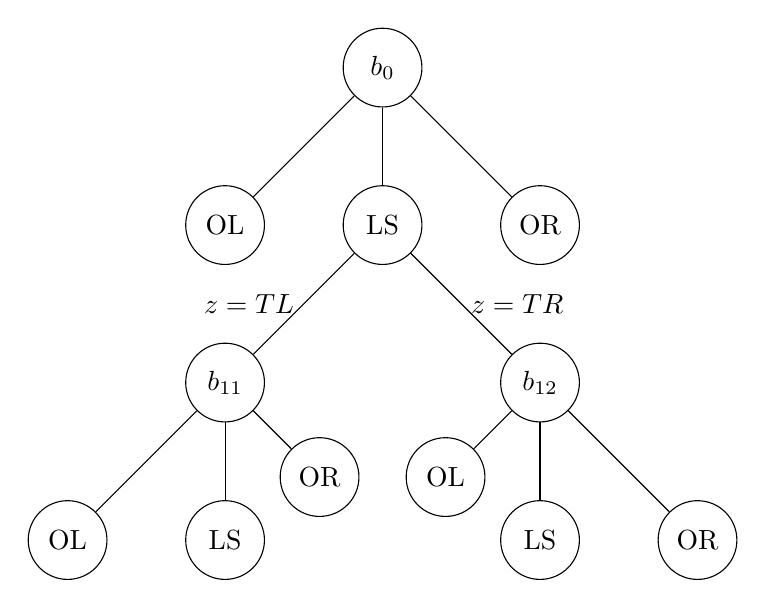
\begin{tikzpicture}
\node[state] (A) {$b_0$};
\node[state] (B) [below left=of A] {OL};
\node[state] (C) [below =of A] {LS};
\node[state] (D) [below right=of A] {OR};
\node[state] (E) [below left=of C]{$b_{11}$};
\node[state] (F) [below left=of E] {OL};
\node[state] (G) [below =of E] {LS};
\node[state] (H) [below right=1.2cm and 1.2cm of E] {OR};
\node[state] (I) [below right=of C]{$b_{12}$};
\node[state] (J) [below left=1.2cm and 1.2cm of I] {OL};
\node[state] (K) [below =of I] {LS};
\node[state] (L) [below right=of I] {OR};
\path[]
    (A) edge node{} (B)
        edge node{} (C)
        edge node{} (D)
    (C) edge node[left] {$z=TL$} (E)
        edge node[right] {$z=TR$} (I)
    (E) edge node{} (F)
        edge node{} (G)
        edge node{} (H)
    (I) edge node{} (J)
        edge node{} (K)
        edge node{} (L);
\end{tikzpicture}    
\end{center}
It is given that $b_0=0.5$. 
From Q2, we also know that $b_{11}=0.85,b_{12}=0.15$.
Then $V(b_{11}),V(b_{12})$ can be calculated
\[V(b_{11})=\max\{-1,-110(0.85)+10,110(0.85)-100\}=-1\]
\[V(b_{12})=\max\{-1,-110(0.15)+10,110(0.15)-100\}=-1\]
With $b_0=0.5$, either observation $z=TL,TR$ is equally likely when $a=LS$,
so 
\[p(z|b_0,a=LS)=b_0=0.5\]
Then $Q(b_0,a=LS)$ can be calculated
\begin{equation}
\begin{aligned}
    Q(b_0,a=LS)
    &=-1+\sum_{z\in Z}p(z|b_0,a=LS)V(b')\\
    &=-1+0.5(-1-1)\\
    &= -2
\end{aligned}
\end{equation}
We also have
\[Q(b_0,a=OL)=-110(0.5)+10=-45\]
\[Q(b_0,a=OR)=110(0.5)-100=-45\]
So
\[V(b_0)=\max_a Q(b_0,a)=\max\{-2,-45,-45\}=-2\]
and the optimal policy would have
\[\pi(b_0)=\argmax_a Q(b_0,a)=LS\]
\[\pi(b_{11})=\argmax_a Q(b_{11},a)=LS\]
\[\pi(b_{12})=\argmax_a Q(b_{12},a)=LS\]


% \begin {tikzpicture}
% \node[state] (A) {LS};
% \node[state] (B) [below left=of A] {LS};
% \node[state] (C) [below right=of A] {OL};
% \path[]
%     (A) edge node[left] {$z=TL$} (B)
%         edge node[right] {$z=TR$} (C);
% \end{tikzpicture}

%======================================
\newpage
\section{QMDP Navigation}

\subsection{Q-Value}
Let $T,B,L,R,M$ denote $Top,Bottom,Left,Right,Middle$ for the cells
so that
\[S=\{TL,TM,TR,ML,MM,MR,BL,BM,BR\}\]
The initial belief $b$ has
\[b(BR)=0.6,b(BM)=0.1,b(MR)=0.3\]
and $b(s)=0$, for $s\notin \{BR,BM,MR\}$.\\
Since $R_S(s)=0$ for all states $s$ where $b(s)>0$, then
\begin{equation}
\begin{aligned}
    \sum_{s\in S}R(s,a)b(s)&=\sum_{s\in S}R_A(a)b(s)\\
    &=\sum_{s\in S}-2b(s)\\
    &= -2
\end{aligned}
\end{equation}
We can calculate
\begin{equation}
\begin{aligned}
    Q_{MDP}(s,a)
    &=\sum_{s\in S} 
    \left(R(s,a)b(s)+\gamma\sum_{s'\in S}p(s'|s,a)V_{MDP}(s')b(s)\right)\\
    &=-2 + \gamma \sum_{s,s'\in S} p(s'|s,a)V_{MDP}(s')b(s)
\end{aligned}
\end{equation}
since there is only one possible next state $s'\in S$,
for each state-action pair $s,a$.\\
Note that $p(s'=s_i|s,a)=1\rightarrow p(s'\neq s_i|s,a)=0$.

\subsubsection{UP}
The state transitions can be determined,
\[p(s'=MR|s=BR,a=UP)=1\]
\[p(s'=MM|s=BM,a=UP)=1\]
\[p(s'=TR|s=MR,a=UP)=1\]
Then
\begin{equation}
\begin{aligned}
    Q_{MDP}(s,a) 
    &=-2 + \gamma \sum_{s,s'\in S} p(s'|s,a)V_{MDP}(s')b(s)\\
    &= -2 + \gamma(V_{MDP}(MR)b(BR)+V_{MDP}(MM)b(BM)+V_{MDP}(TR)b(MR))\\
    &= -2 + \gamma(4\times 0.6 -20\times 0.1+6\times 0.3)\\
    &= -2 + 2.2\gamma
\end{aligned}
\end{equation}

\subsubsection{DOWN}
\[p(s'=BR|s=BR,a=DOWN)=1\]
\[p(s'=BM|s=BM,a=DOWN)=1\]
\[p(s'=BR|s=MR,a=DOWN)=1\]
Then
\begin{equation}
\begin{aligned}
    Q_{MDP}(s,a) 
    &=-2 + \gamma \sum_{s,s'\in S} p(s'|s,a)V_{MDP}(s')b(s)\\
    &= -2 + \gamma(V_{MDP}(BR)b(BR)+V_{MDP}(MM)b(BM)+V_{MDP}(BR)b(MR))\\
    &= -2 + \gamma(2\times 0.6 +4\times 0.1+2\times 0.3)\\
    &= -2 + 2.2\gamma
\end{aligned}
\end{equation}

\subsubsection{LEFT}
\[p(s'=BM|s=BR,a=LEFT)=1\]
\[p(s'=BL|s=BM,a=LEFT)=1\]
\[p(s'=MM|s=MR,a=LEFT)=1\]
Then
\begin{equation}
\begin{aligned}
    Q_{MDP}(s,a) 
    &=-2 + \gamma \sum_{s,s'\in S} p(s'|s,a)V_{MDP}(s')b(s)\\
    &= -2 + \gamma(V_{MDP}(BM)b(BR)+V_{MDP}(BL)b(BM)+V_{MDP}(MM)b(MR))\\
    &= -2 + \gamma(4\times 0.6 +6\times 0.1-20\times 0.3)\\
    &= -2 - 3\gamma
\end{aligned}
\end{equation}

\subsubsection{RIGHT}
\[p(s'=BR|s=BR,a=RIGHT)=1\]
\[p(s'=BR|s=BM,a=RIGHT)=1\]
\[p(s'=MR|s=MR,a=RIGHT)=1\]
Then
\begin{equation}
\begin{aligned}
    Q_{MDP}(s,a) 
    &=-2 + \gamma \sum_{s,s'\in S} p(s'|s,a)V_{MDP}(s')b(s)\\
    &= -2 + \gamma(V_{MDP}(BR)b(BR)+V_{MDP}(BR)b(BM)+V_{MDP}(MR)b(MR))\\
    &= -2 + \gamma(2\times 0.6 +2\times 0.1+4\times 0.3)\\
    &= -2 + 2.6\gamma
\end{aligned}
\end{equation}

\subsection{Best Action}
\[\pi_{QMDP}(b)=\argmax_a Q_{MDP}(b,a)=RIGHT\]
The best action is $a=RIGHT$.

%======================================
\newpage
\bibliographystyle{abbrv}
\bibliography{ref}

\end{document}